  %%%%%%%%%%%%%%%%%%%%%%%%%%%%%%%%%%%%%%%%%

% Short Sectioned Assignment
% LaTeX Template
% Version 1.0 (5/5/12)
%
% This template has been downloaded from:
% http://www.LaTeXTemplates.com
%
% Original author:
% Frits Wenneker (http://www.howtotex.com)
%
% License:
% CC BY-NC-SA 3.0 (http://creativecommons.org/licenses/by-nc-sa/3.0/)
%
%%%%%%%%%%%%%%%%%%%%%%%%%%%%%%%%%%%%%%%%%

%----------------------------------------------------------------------------------------
%   PACKAGES AND OTHER DOCUMENT CONFIGURATIONS
%----------------------------------------------------------------------------------------

%\documentclass[paper=a4, fontsize=11pt]{scrartcl} % A4 paper and 11pt font size
\documentclass{article}
\usepackage[T1]{fontenc} % Use 8-bit encoding that has 256 glyphs
\usepackage{palatino} % Use the Adobe Utopia font for the document - comment this line to return to the LaTeX default
\usepackage[english]{babel} % English language/hyphenation
\usepackage{amsmath,amsfonts,amsthm} % Math packages
\usepackage{multicol,lastpage,fullpage,framed,fancybox,enumerate,tikz}
\usepackage{lipsum} % Used for inserting dummy 'Lorem ipsum' text into the template
\usepackage{mathrsfs}
\usepackage{graphicx}
\usepackage{mathtools}
\usepackage{multirow}
\usepackage{algorithm}
\usepackage{algpseudocode}

\usepackage{color}   %May be necessary if you want to color links
\usepackage{hyperref}
\hypersetup{
    colorlinks=true, %set true if you want colored links
    linktoc=all,     %set to all if you want both sections and subsections linked
    linkcolor=blue,  %choose some color if you want links to stand out
}

%
%
%
%   A T T E N T I O N ! ! !
%
%   SET YOUR GRAPHICS FOLDER IN THE LINE BELOW
%
\graphicspath{ {.} }
\usepackage{sectsty} % Allows customizing section commands
\allsectionsfont{\centering \normalfont\scshape} % Make all sections centered, the default font and small caps

\usepackage{fancyhdr} % Custom headers and footers
\pagestyle{fancy plain} % Makes all pages in the document conform to the custom headers and footers
\fancyhead[L]{\textsc{CSEN 5830}}
\fancyhead[R]{\textsc{Final Project Report}} % No page header - if you want one, create it in the same way as the footers below
\fancyfoot[L]{} % Empty left footer
\fancyfoot[C]{} % Empty center footer
\fancyfoot[C]{- \thepage -} % Page numbering for right footer
\renewcommand{\headrulewidth}{0.5pt} % Remove header underlines
\renewcommand{\footrulewidth}{0pt} % Remove footer underlines
\setlength{\headheight}{13.6pt} % Customize the height of the header

\fancypagestyle{noheader}{    %create style that allows to skip header manually on pages with new section
    \fancyhead{}
    \renewcommand{\headrulewidth}{0pt}
}

\numberwithin{equation}{section} % Number equations within sections (i.e. 1.1, 1.2, 2.1, 2.2 instead of 1, 2, 3, 4)
\numberwithin{figure}{section} % Number figures within sections (i.e. 1.1, 1.2, 2.1, 2.2 instead of 1, 2, 3, 4)
\numberwithin{table}{section} % Number tables within sections (i.e. 1.1, 1.2, 2.1, 2.2 instead of 1, 2, 3, 4)

\setlength\parindent{0pt} % Removes all indentation from paragraphs - comment this line for an assignment with lots of text

%----------------------------------------------------------------------------------------
%   TITLE SECTION
%----------------------------------------------------------------------------------------

\newcommand{\horrule}[1]{\rule{\linewidth}{#1}} % Create horizontal rule command with 1 argument of height

\title{
\normalfont \LARGE
\textsc{University of Colorado at Boulder} \\ [25pt] % Your university, school and/or department name(s)
\textsc{COEN 5830 - ROBO 5000} \\ [20pt]
\textsc{Fall 2024} \\ [20pt]
\textsc{Professor: Dr. Leo Beuken} \\ [12pt]
\textsc{Teaching Assistant: Srikrishna Raghu} \\ [12pt]
\horrule{1pt} \\[0.4cm] % Thin top horizontal rule
\huge Final Project \\ % The assignment title
\horrule{1pt} \\[0.6cm] % Thick bottom horizontal rule
}

\author{
  \textsc{ Team Members:} \\ [4 mm]
  \textsc{ Ian Mcconachie}\\[2mm]
  \textsc{ Michael Bernabei}\\[2mm]
}

\date{\normalsize\today} % Today's date or a custom date

\begin{document}

\maketitle % Print the title
\thispagestyle{empty} %make title page header empty
\newpage




\tableofcontents
\listofalgorithms

\newpage

%----------------------------------------------------------------------------------------
%   PROBLEM SECTION
%----------------------------------------------------------------------------------------
%

\section{Problems Attempted}
\\~\\
\begin{center}
 \begin{minipage}{.4\textwidth}
 \begin{itemize}
    \item \hyperref[sec:Perception]{Perception - Lidar Occupancy Grid}
    \item \hyperref[sec:SensorFusion]{Perception - IMU Sensor Fusion}
    \item \hyperref[sec:CannyEdge]{Perception - Canny Edge Detection }
    \item \hyperref[sec:RRT]{Path Planning - RRT - 3 points }
    \item \hyperref[sec:DynAndCtrl]{Dynamics And Control - 5.1 Part A }
 \end{itemize}
 \end{minipage}
\end{center}


\newpage


\section{Perception}

\begin{framed}
\subsection{Lidar Occupancy Grid}
\label{sec:Perception}

\textbf{ Lidar Occupancy Grid - 2 points} \\

For the lidar occupancy grid problem we elected to use the \textbf{Brensenham Line Algorithm} to rasterize the rays throughout the environment.  We chose this method after Dr. Leo highlighted the benefits of the line algorithm for rasterizing rays.  One particularly amazing feature of the algorithm is the use of only integer arithmetic in the calculation of occupancies.  Using only integer calculations in the occupancies reduces computationally complexity and therefore increases speed. Now since Brensenham's line algorithm is the heart of our work, we will describe the steps in our implemention that lead up to and after the Brensenham portion of our code.

\subsubsection{Lidar Occupancy Algorithm High-level Steps}
In this section we will highlight the main steps in our algorithm for this part of the project. We will try to stick to plain old english when describing these steps and save coding details for the oral exam portion of this project.

 
\begin{algorithm}[H]
\caption{Lidar Occupancy Grid Algorithm}\label{alg:cap}
\begin{algorithmic}[1] % Enable number with [1]
\State Read in lidar, heading, and position data then store in internal data structures
\State Create Grid based off passed in lidar CSV data 
\State Start animation loop
\While {True}
\State Convert incoming lidar readings and robot position data to grid coordinates
\State Mark current position of robot on grid 
\State Rasterize lidar readings using Brensenham's line algorthim and update grid
\State Rescale grid x,y axis to real world x,y axis
\State display animation, i.e. show state of lidar scan to user
\EndWhile
\end{algorithmic}
\end{algorithm}

The above algorithm highlights the main steps in the occupancy grid algorithm.  As previously stated, code details will be highlighted upon request at the oral examination.


\end{framed}


\begin{framed}
\subsection{IMU Sensor Fusion}
\label{sec:SensorFusion}
\textbf{IMU Sensor Fusion - 1 points} \\
\end{framed}


\begin{framed}
\subsection{Canny Edge Detection - 1 + 1 Bonus Point}
\label{sec:CannyEdge}
\textbf{ Canny Edge Detection - 1 Point + 1 Bonus Point} \\
For Canny edge detection, we implemented each of the steps necessary for the algorithm and then compared our results with those of OpenCV.  We noticed that OpenCV's implementation of the Canny edge detection algorithm was much faster and yielded better results.  We attribute this to years of optimization under the hood and more eye's looking at their Canny edge implementation code.  We noticed that tuning our low and high thresholds in the hystersis step would yield better or worse results depending on how we tuned the thresholds. We feel OpenCV has a clever way to select these values and therefore yeild better results.

\begin{algorithm}[H]
\caption{Simple Canny Edge Implementation}\label{alg:cap}
\begin{algorithmic}[1] % Enable number with [1]
\State Load color image 
\State Convert loaded image to gray scale image
\State Apply Gaussian blur to gray scale image to reduce noise
\State Apply non-maximum suppression to then edges
\State Perform depth first search hysteresis thresholding
\end{algorithmic}
\end{algorithm}

In the image below, we have our implementation of Canny.  Each of the sub-images correspond to the steps in the previously mentioned algorithm. Our implementation does a fairly good job of detecting the lines in the image.   

\begin{center}
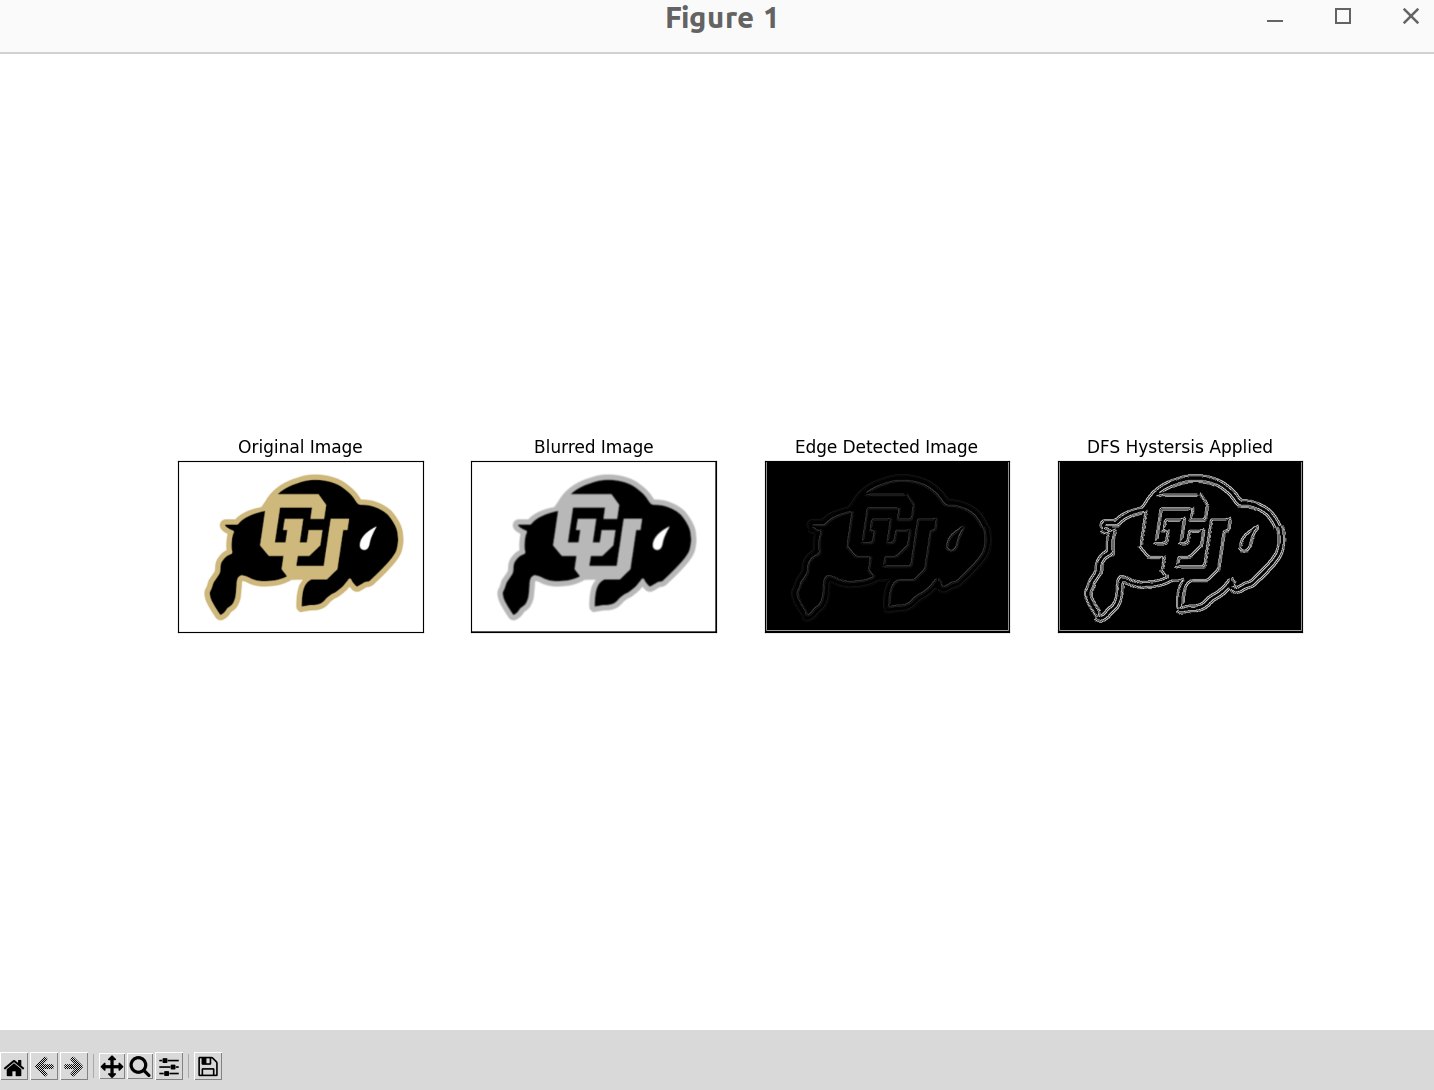
\includegraphics[scale=.25]{ourCanny.png}
\end{center}

However, in the image below, we see OpenCV's Canny implementation and notice their final image looks better.  Again, we believe this is some optimizations made in their hystersis step.

\begin{center}
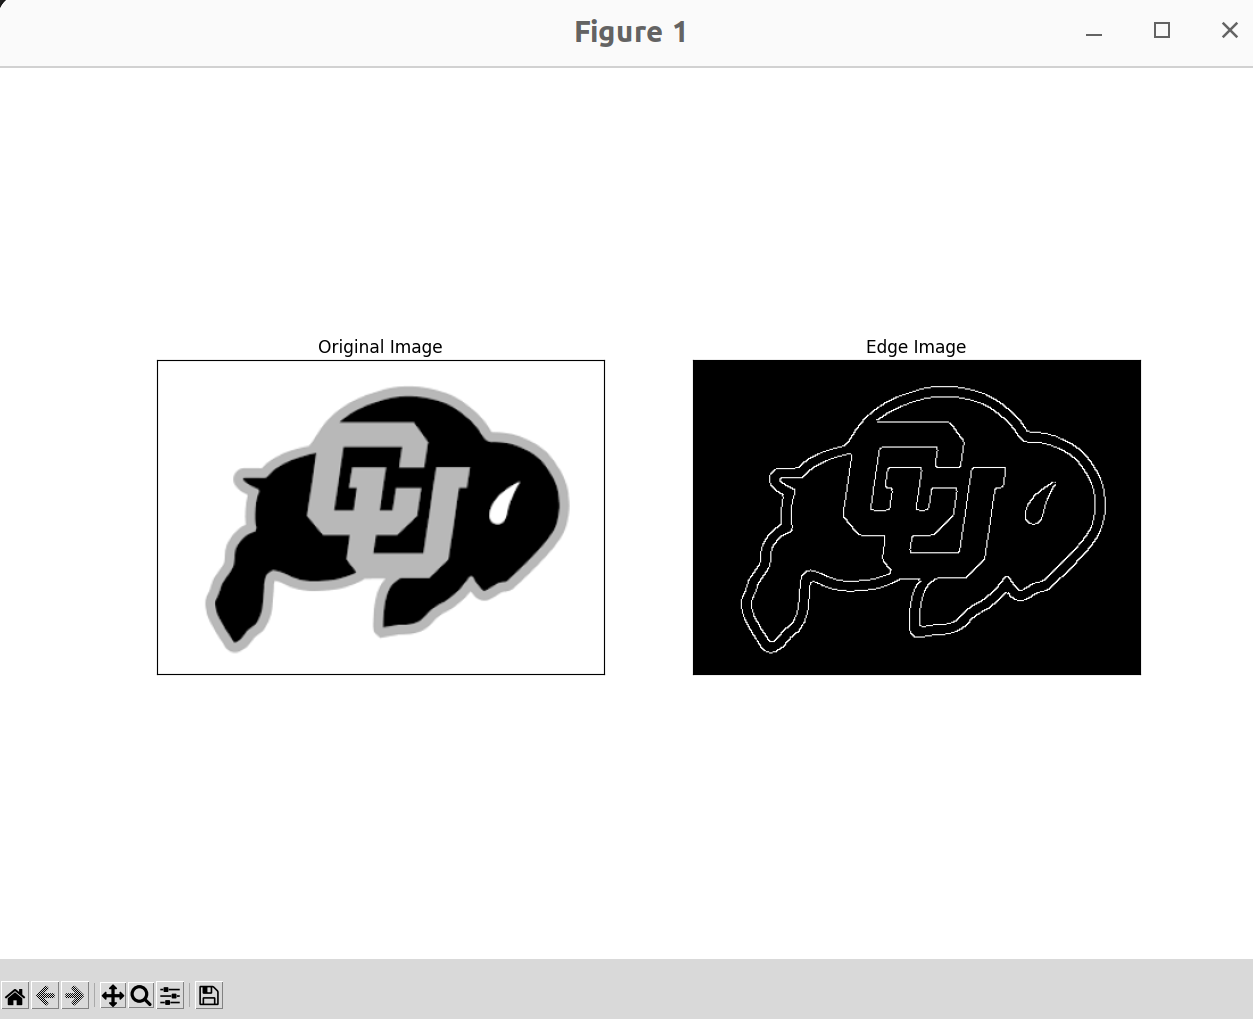
\includegraphics[scale=.25]{thierCanny.png}
\end{center}

Finally, to ensure we get credit for the bonus point.  It is important to note that we implemented a DFS using a stack and while loop to perform the hystersis step in the Canny edge detection algorithim.

\end{framed}


\section{Path Planning}

\begin{framed}
\subsection{ RRT - 3 points}
\label{sec:RRT}
\end{framed}

\section{Dynamics and Control}

\begin{framed}
\subsection{ Part A - 2 Points}
\label{sec:DynAndCtrl}
\end{framed}


\end{document}